%! Author = jonathan
%! Date = 5/27/25
\chapter{Evaluation}\label{ch:evaluation}
\begin{table}[h]
    \centering
    \caption{Implementation metrics of~\sysname using fully inlined NVSHMEM.}
    \label{tab:impl_metrics}
    \begin{tabular}{cc}
        \toprule
        \textbf{Metric} & \textbf{Value}\\ \hline
        Total lines of code (CUDA/C++) & 6820 \\
        Kernel stack frame size & 0 B \\
        Spill stores (per thread) & 0 \\
        Spill loads (per thread) & 0 \\
        Shared memory usage (per block) & 46 KB \\
        Registers per thread & 255 \\
        Max active blocks per SM & 2 \\
        Compilation time & 53 seconds \\
        Binary size & 29 MB\\
    \end{tabular}
\end{table}
We implement (\S\ref{tab:impl_metrics}) and evaluate \sysname and evaluate across
five metrics: \textbf{Forward Latency} (\S~\ref{sec:forward-latency}),
\textbf{GPU Utilization} (\S~\ref{sec:gpu-utilization}),
\textbf{Overlap Efficiency} (\S~\ref{sec:overlap-efficiency}),
\textbf{Throughput} (\S~\ref{sec:throughput}), and \textbf{Expert Scalability} (\S~\ref{sec:expert-scalability}).
\section{Setup}\label{sec:setup}
We run experiments on a server with 8 NVIDIA H100 80G GPUs interconnected via NVLink,
125 GB of RAM, and 20 vCPUs. We used PyTorch 2.6.0, CUDA 12.8, and Ubuntu 22.04.
All experiments use MoE transformer models configured with 16 attention heads,
an embedding dimension of 2048, and an FFN intermediate size of 2048.
We apply Distributed Data Parallelism (DDP) and Expert Parallelism for all experiments.
We execute only the forward pass over a single MoE layer and measure the average runtime
of 32 passes after 32 warmup passes.
We use top-2 routing with a capacity factor of 1.0.
We compare \sysname against several state-of-the-art MoE systems:
(1) \textbf{Comet}~\cite{comet},
(2) \textbf{FasterMoE}~\cite{fastermoe},
(3) \textbf{Megatron-CUTLASS}~\cite{megatron-lm}, and
(4) \textbf{Megatron-TE}: Megatron-LM with Transformer Engine~\cite{transformer-engine}.
Comet relies on~\verb|cudaMemcpyPeerAsync|~\cite{fluxp2p}, while FasterMoE and Megatron-LM use NCCL exclusively for communication.
We also evaluate \sysname on a multi-node environment and discuss our findings in \S\ref{sec:multi-node-evaluation}.
\subsection{Desiderata}\label{subsec:desiderata}
In our experiments, we observe Comet exhibiting anomalously bad performance values at 8 GPUs,
so we exclude their results from evaluations at 8 GPUs and only include for results at $\leq$
4 GPUs.
\textbf{Note} we evaluate \sysname using FP32 precision whereas all baselines use FP16.
We do so because (1) no baseline supports FP32 and (2) time constraints prevent us from tuning our system
to peak performance at FP16.
Most importantly, this precision discrepancy disadvantages \sysname by doubling the
communication and computation precision, \emph{making our results a conservative lower bound}.
Yet, as we show in the succeeding sections, \sysname outperforms all baselines.
\section{Forward Latency}\label{sec:forward-latency}
\begin{figure}[!h]
    \centering
    \begin{subfigure}{0.49\textwidth}
        \centering
        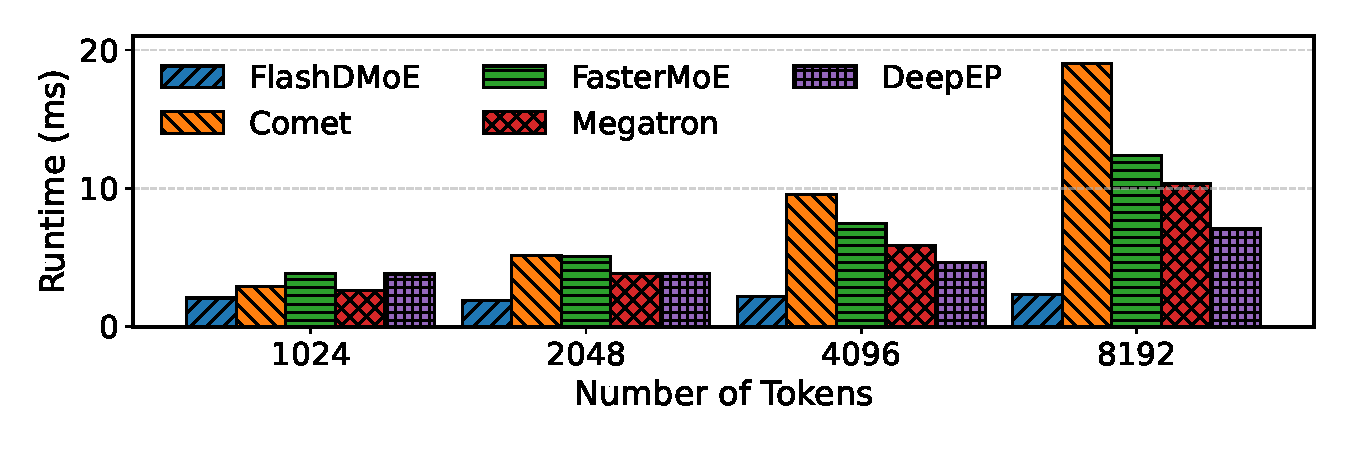
\includegraphics[width=\linewidth, keepaspectratio]{figures/scaling_tokens}
        \caption{4 H100s}
        \label{sub:4gl}
    \end{subfigure}
    \begin{subfigure}{0.49\textwidth}
        \centering
        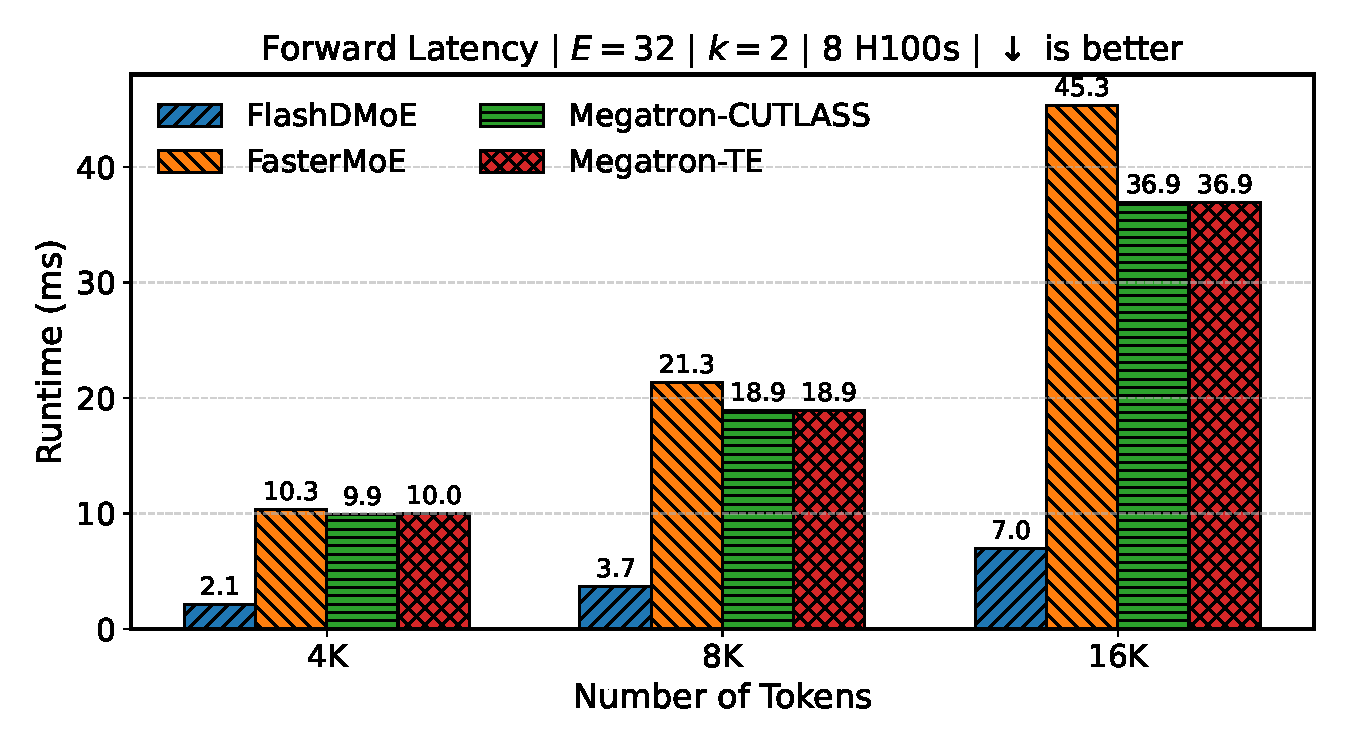
\includegraphics[width=\linewidth, keepaspectratio]{figures/scaling_tokens_8}
        \caption{8 H100s}
        \label{sub:8gl}
    \end{subfigure}
    \caption{Forward Latency as the \emph{Number of Tokens} per GPU increases.}
    \label{fig:fl}
\end{figure}
We first measure the forward latency of FlashDMoE across different sequence lengths on both 4 and 8 GPU setups
(Figure~\ref{fig:fl}).
FlashDMoE consistently outperforms all baselines,
with especially notable improvements at longer sequence lengths.
On 4 GPUs, it achieves up to \textbf{4.6}x speedup over Megatron-TE at 16K tokens,
and \textbf{2.6}x over FasterMoE.
The gains are even more pronounced at 8 GPUs
where FlashDMoE maintains low latency, exhibiting up to \textbf{6.4}x speedup over baselines that
degrade steeply due to increasing communication costs as token buffers increase proportionally.
These results highlight FlashDMoE’s ability to scale token throughput without suffering from the communication
penalties that plague other implementations.
\section{GPU SM Utilization}\label{sec:gpu-utilization}
\begin{figure}[!ht]
    \centering
    \centering
    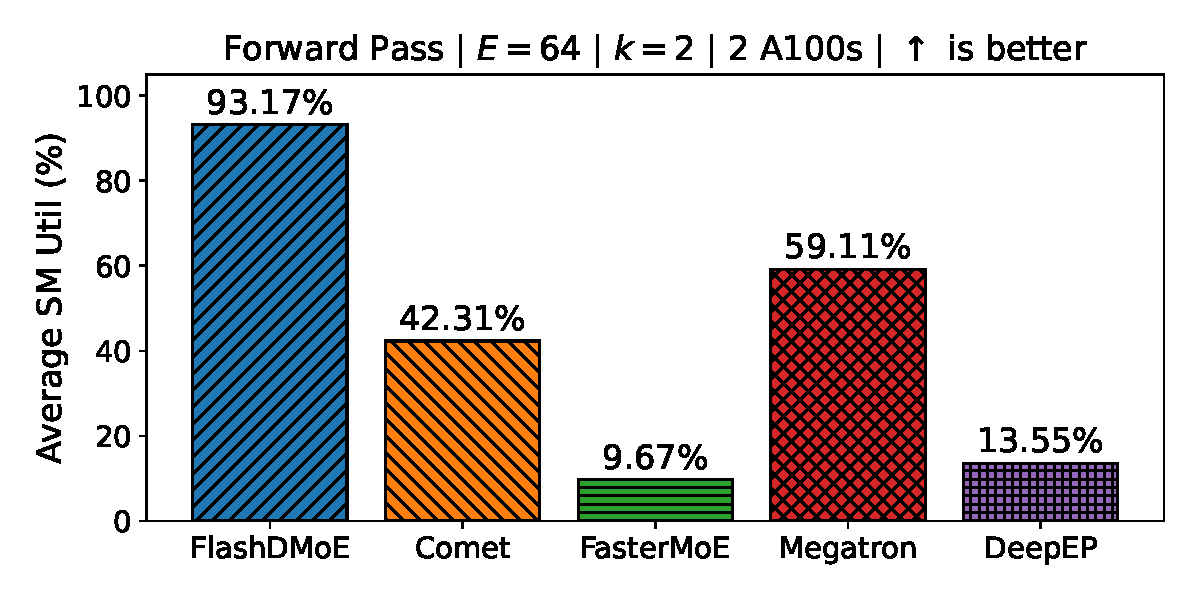
\includegraphics[width=0.8\linewidth, keepaspectratio]{figures/sm_util}
    \caption{Comparison of SM utilization, defined as the ratio of cycles in which SMs
    have at least one warp in flight
    to the total number of cycles~\cite{nsight-metrics}.
    Values represent the average SM utilization over 100 iterations.
    All experiments use T = 8K and E = 64 on two A100s}
    \label{fig:smu}
\end{figure}
To quantify GPU efficiency, we measure Streaming Multiprocessor (SM) utilization during the forward pass (Figure~\ref{fig:smu}).
FlashDMoE achieves 93.17\% average SM utilization,
over \textbf{9}x higher than FasterMoE (9.67\%), \textbf{6.8}x higher than DeepEP+Megatron-LM (13.55\%)
\textbf{4}x higher than Megatron-TE (59.11\%), and
\textbf{2.2}x higher than Comet (42.31\%).
This improvement stems from our fully fused kernel architecture and
fine-grained pipelining of compute and communication tasks.
By eliminating idle gaps due to kernel launches and enabling in-kernel task scheduling,
FlashDMoE ensures SMs remain busy with productive work throughout execution.
\section{Overlap Efficiency}\label{sec:overlap-efficiency}
\begin{figure}[!h]
    \centering
    \begin{subfigure}{0.49\textwidth}
        \centering
        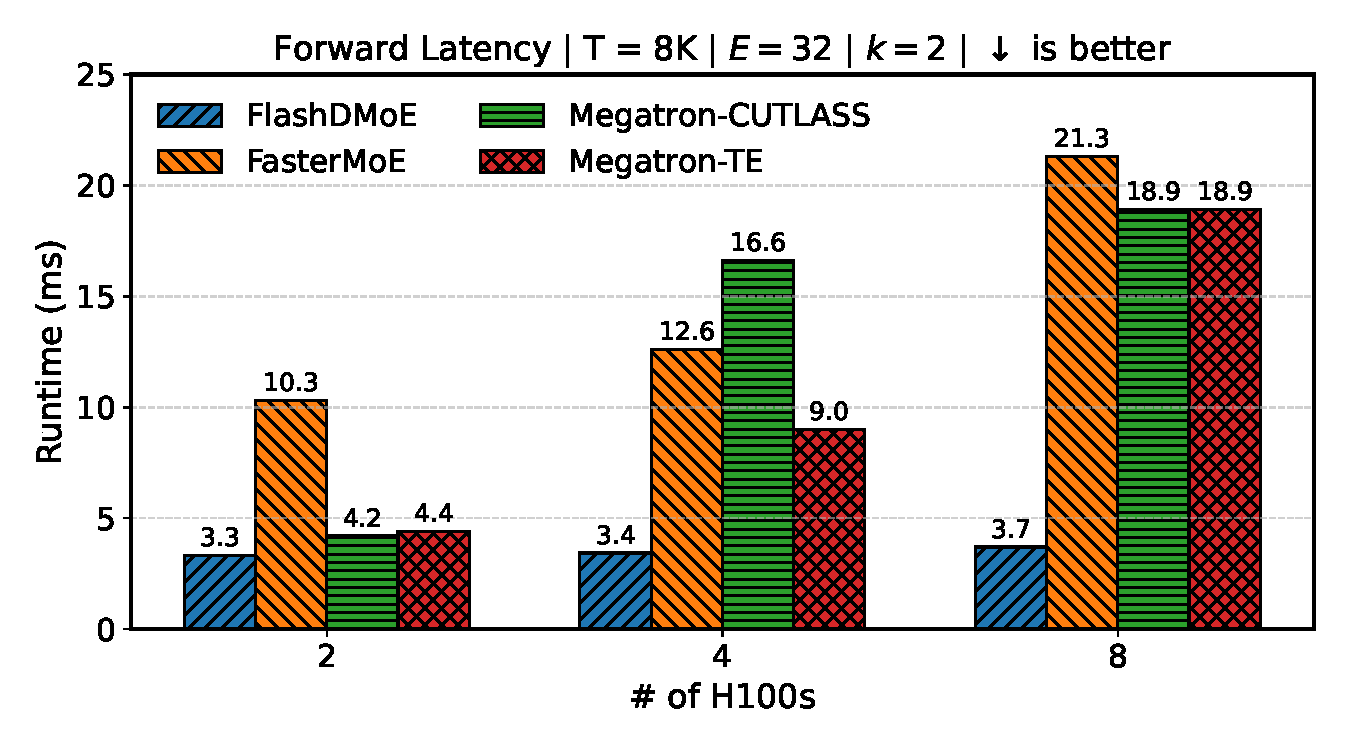
\includegraphics[width=\linewidth, keepaspectratio]{figures/scaling_gpus_8}
        \caption{Latency as Number of GPUs increases.}
        \label{fig:lng}
    \end{subfigure}
    \begin{subfigure}{0.49\textwidth}
        \centering
        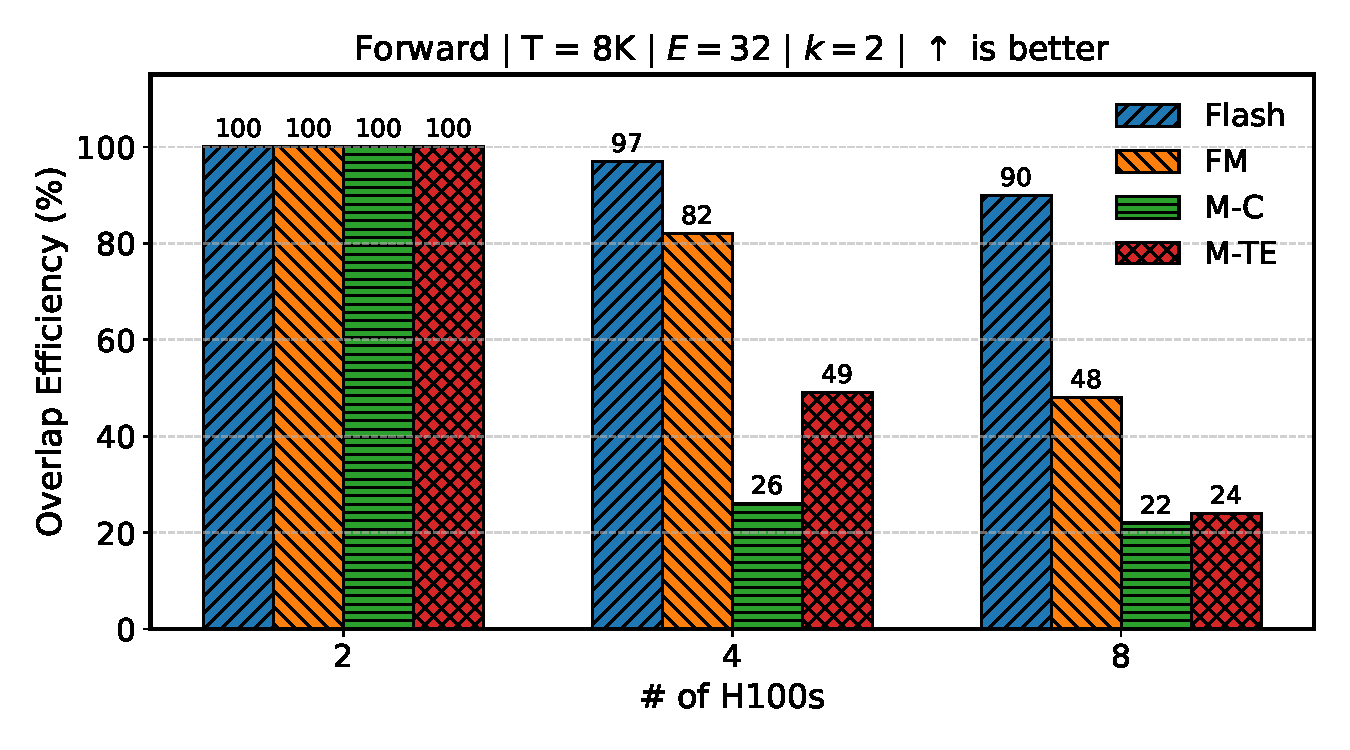
\includegraphics[width=\linewidth, keepaspectratio]{figures/overlap_efficiency_8}
        \caption{Weak scaling efficiency.}
        \label{fig:oe}
    \end{subfigure}
    \caption{Forward Latency as the \emph{Number of Tokens} per GPU increases. We define Overlap Efficiency $O_e$
        to be $O_e = T(2) / T(N_G)$, where $T(N_G)$ is the latency at $N_G$ GPUs and $T(2)$ is the latency at 2 GPUs.}
    \label{fig:oet}
\end{figure}
We evaluate the extent to which \sysname overlaps communication and computation by measuring weak scaling efficiency
as the number of GPUs increases (Figure~\ref{fig:oe}).
We note that most baselines fail to execute at a single GPU, hence why we use 2 GPUs as the reference point.
We observe that Megatron-CUTLASS and Megatron-TE degrade significantly,
with overlap efficiency dropping below 0.5 at $\geq 4$ GPUs. \sysname gives up to \textbf{3.88}x and
\textbf{4}x higher efficiency at 4 and 8 GPUs, respectively.
Figure~\ref{fig:lng} further illuminates this efficiency, as \sysname shows stable forward latency growth,
whereas baselines Megatron-CUTLASS and Megatron-TE experience approximately linear
latency amplification while FasterMoE exhibits sublinear scaling.
We attribute this suboptimal performance to straggler effects and exposed communication.
In contrast, \sysname demonstrates uniform latency as expected since the workload per
GPU is fixed in this weak scaling experiment.
These results further corroborate that \sysname's actor-based design and asynchronous data movement
achieve near-ideal overlap, even at scale.
\section{Throughput}\label{sec:throughput}
\begin{figure}[!ht]
    \centering
    \centering
    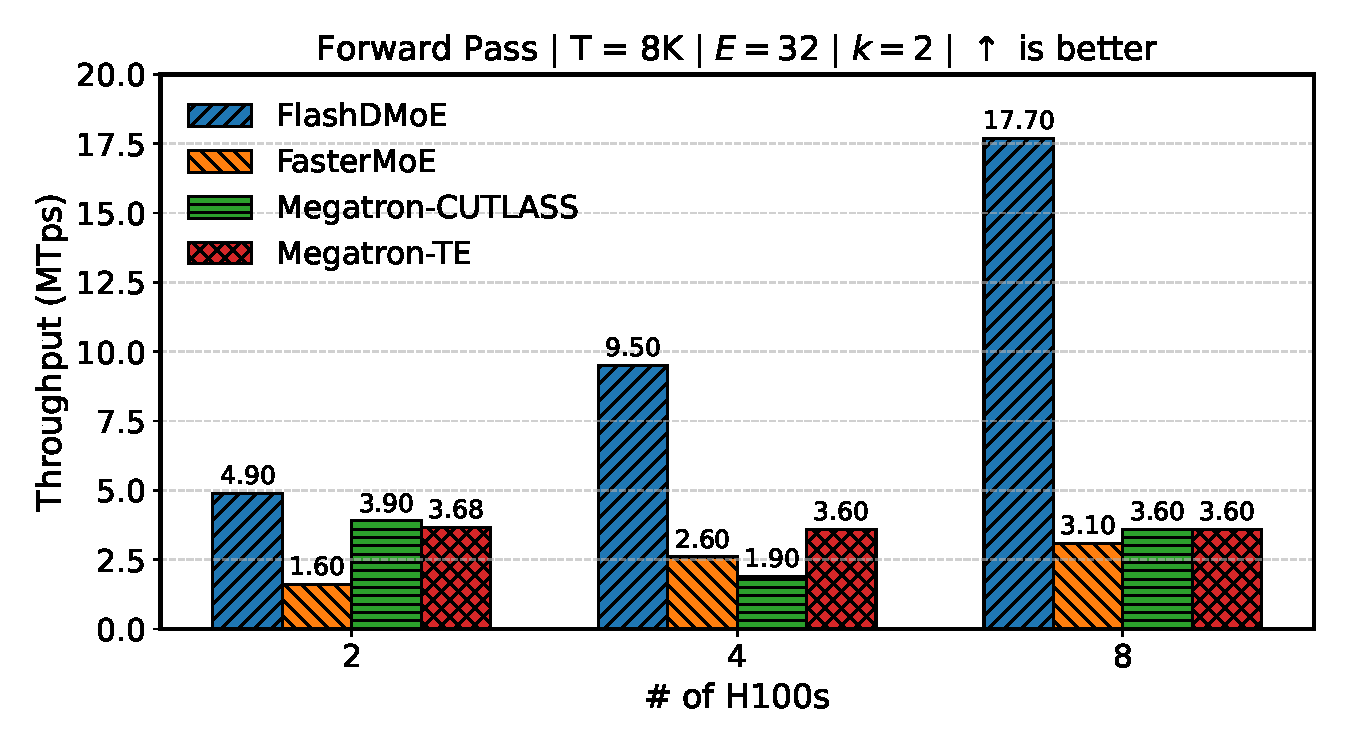
\includegraphics[width=0.7\linewidth, keepaspectratio]{figures/throughput_8}
    \caption{Throughput as the amount of GPUs increases. We compute throughput as $\frac{T * N_G}{latency}$, where
        $N_G$ is the number of GPUs.}
    \label{fig:thr}
\end{figure}
Throughput, measured in tokens per second (MTokens/s), reflects end-to-end system efficiency.
As shown in Figure~\ref{fig:thr}, \sysname
scales linearly with GPU count,
reaching 17.7 MTokens/s at 8 GPUs.
This is over \textbf{5.7}x higher than FasterMoE and \textbf{4.9}x higher than Megatron-TE and Megatron-CUTLASS\@.
Notably, these results are achieved despite \emph{FlashDMoE operating entirely in FP32,
    while baselines use FP16}.
This indicates that FlashDMoE’s design eliminates throughput bottlenecks not by
exploiting lower precision, but by maximizing hardware utilization and eliminating host-driven inefficiencies.
\section{Expert Scalability}\label{sec:expert-scalability}
\begin{figure}[!h]
    \centering
    \begin{subfigure}{0.49\textwidth}
        \centering
        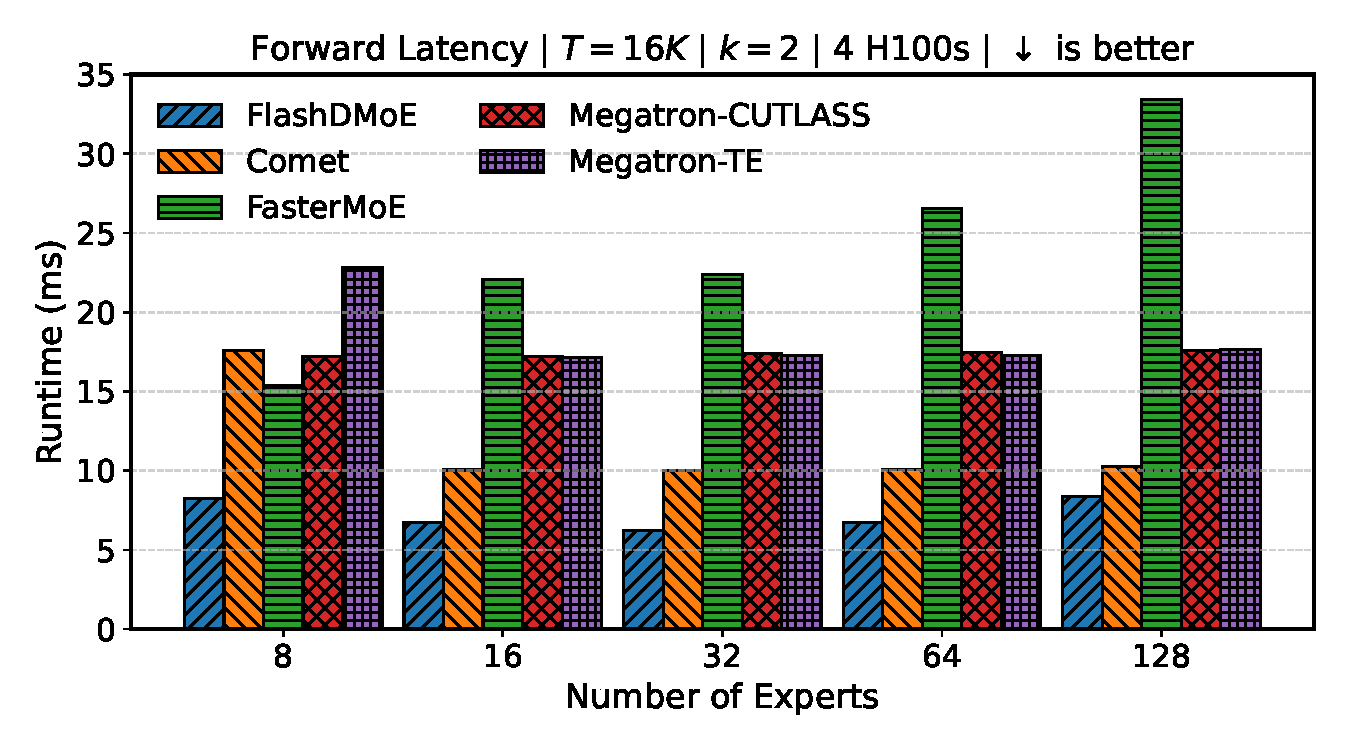
\includegraphics[width=\linewidth, keepaspectratio]{figures/scaling_experts}
        \caption{4 H100s}
        \label{sub:4gx}
    \end{subfigure}
    \begin{subfigure}{0.49\textwidth}
        \centering
        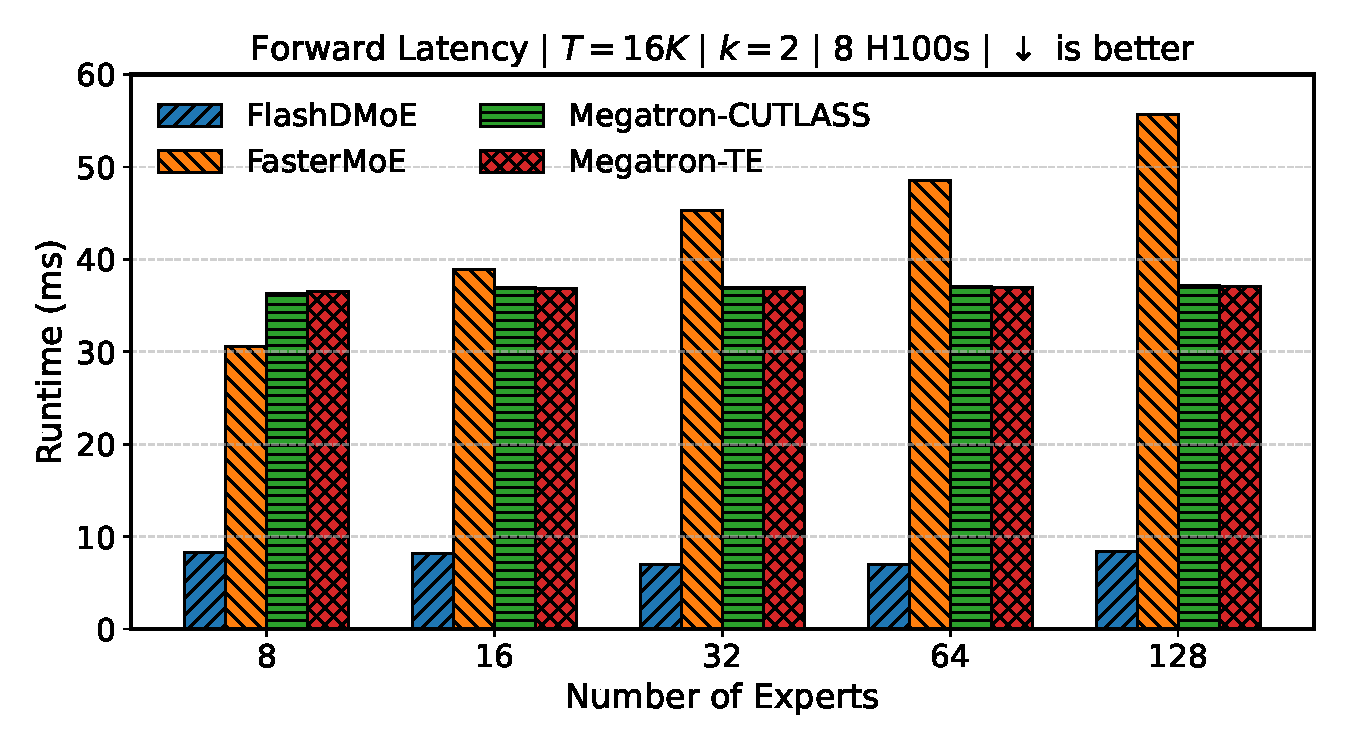
\includegraphics[width=\linewidth, keepaspectratio]{figures/scaling_experts_8}
        \caption{8 H100s}
        \label{sub:8gx}
    \end{subfigure}
    \caption{Forward Latency as the \emph{Number of experts} increases.}
    \label{fig:xs}
\end{figure}
We analyze how \sysname scales with increasing number of experts at fixed sequence length (T = 16K).
Note that for the discussed plots, the number of experts on the x-axis is the \emph{total number across all GPUs}.
Each GPU gets 1/8th of this value.
As seen in Figure\ref{fig:xs}, \sysname maintains \emph{low, uniform} latency, as desired,
even as the number of experts grows from 8 to 128.
In contrast, baselines exhibit superlinear latency increases due to increased kernel launch overheads.
\sysname outperforms these baselines by up to \textbf{4}X at 4 H100s and \textbf{6.6}X at 8 H100s, both at 128 experts.
\sysname’s payload-efficient communication and scheduler-driven
in-kernel dispatching allow it to sustain expert parallelism
without incurring the communication and orchestration penalties seen in other systems.
These results reinforce FlashDMoE’s scalability for ultra-sparse MoE configurations.
\section{Multi-Node Evaluation}\label{sec:multi-node-evaluation}
In this experiment, we seek to evaluate \sysname in the multi-node setting, where GPU interconnects
span both InfiniBand (internode) and NVLink connections (intranode).
\subsection{Setup}\label{subsec:setup}
We use 4 nodes, where each node comprises 4 A100 GPUs fully interconnected via NVLink.
Across nodes, each GPU uses a single NIC providing 25 GB/s of bandwidth.
We set the number of experts to be $16$ and assign each GPU to host only one,
so the number of local experts is $1$.
Note that we define MIV formally as follows:
\[
    MIV = \frac{Tokens}{Experts} * local\_{experts} * precision * hidden\_size * 2 * n_{rg}
\]
where $n_{rg}$ is the number of remote peers and the multiplicative
factor of $2$ accounts for communication rounds (dispatch and combine).
$n_{rg} = 12$ for this experiment.
\subsection{Results}\label{subsec:results}
\begin{figure} [!ht]
    \centering
    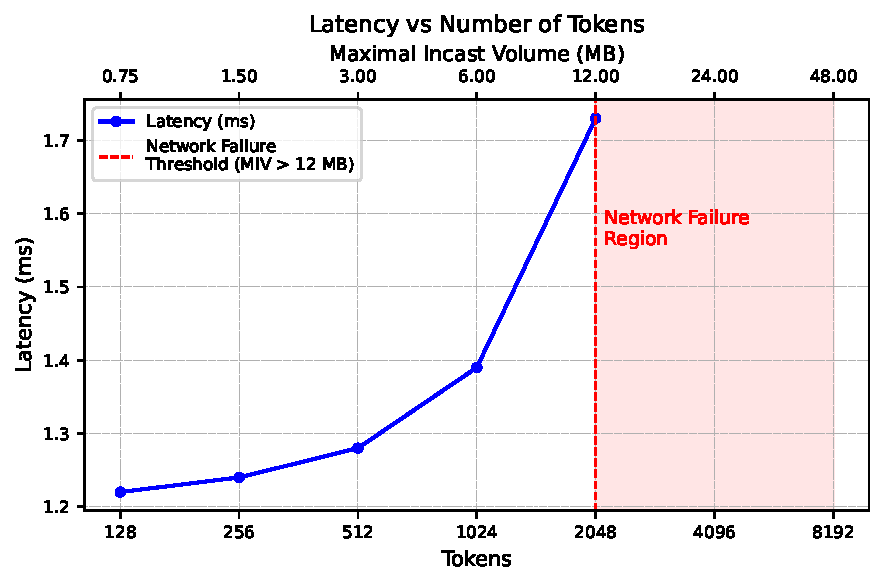
\includegraphics[width=4in,keepaspectratio]{figures/multi_node_fail}
    \caption{Multi-node Latency evaluation.
    Embbeding dimension is $1024$ and FFN intermediate size is $4096$.
    We define Maximal Incast Volume (MIV) as the worst case upper bound for data volume that a
    NIC receives in a single incast occurence.}
    \label{fig:multi_fail}
\end{figure}
We observe a sublinear increase in latency as we scale the number of tokens.
However, we observe at $Tokens > 2048$, that the application fails to terminate
due to failure to receive expectant messages.
We hypothesize this failure to be due to buffer overflow at the networking hardware layer as is common for applications
that generate many and large messages~\cite{nerscNetworkNERSC} like our system.
We note that this failure is addressable by tuning hardware configurations~\cite{ofiwgFi_cxi7} but we consider
this exploration as an exercise orthogonal to this work.
\section{Memory Overhead}\label{sec:eval:memory}
We measure the GPU memory required for the symmetric tensor $L$ and runtime bookkeeping state of \sysname.
Memory overhead depends primarily on the tile size, expert capacity (EC), and the number of experts ($E$).
Table~\ref{tab:memory-overhead} summarizes memory overhead under various configurations, confirming that \sysname maintains a modest and predictable memory footprint.
\begin{table}[!ht]
    \centering
    \caption{Memory overhead with (tile size $bM = 128$), $Size(T) = \text{Tokens} * 4KB$).}
    \label{tab:memory-overhead}
    \setlength{\tabcolsep}{4pt}
    \renewcommand{\arraystretch}{0.9}
    \begin{tabular}{ccccccc}
        \toprule
        \textbf{Tokens} & \textbf{Experts} & \textbf{EC} & \textbf{max(bM, EC)} & \textbf{Bookkeeping (MB)} & $Size(L)$ \textbf{(MB)} & \textbf{Total (MB)} \\
        \midrule
        4K  & 16  & 256  & 256  & 64.57  & 64.00  & 128.57 \\
        4K  & 32  & 128  & 128  & 64.55  & 64.00  & 128.55 \\
        4K  & 64  & 64   & 128  & 128.90 & 128.01 & 256.91 \\
        4K  & 128 & 32   & 128  & 257.96 & 256.02 & 513.98 \\
        \midrule
        8K  & 16  & 512  & 512  & 128.95 & 128.01 & 256.95 \\
        8K  & 32  & 256  & 256  & 128.90 & 128.01 & 256.91 \\
        8K  & 64  & 128  & 128  & 128.90 & 128.01 & 256.91 \\
        8K  & 128 & 64   & 128  & 258.15 & 256.02 & 514.17 \\
        \midrule
        16K & 16  & 1024 & 1024 & 257.89 & 256.02 & 513.90 \\
        16K & 32  & 512  & 512  & 257.79 & 256.02 & 513.81 \\
        16K & 64  & 256  & 256  & 257.80 & 256.02 & 513.81 \\
        16K & 128 & 128  & 128  & 258.53 & 256.02 & 514.54 \\
        \bottomrule
    \end{tabular}
\end{table}
\clearpage